\documentclass[10pt,a4paper]{article}
% This file compiles fine with pdflatex,
% (here: TeX Live 2013/Frankfurt Institute for Advanced Sciences)
\usepackage[utf8]{inputenc}
\usepackage{hyperref}
\hypersetup{linktocpage}
\usepackage[american]{babel}
\usepackage{amsmath} % xrightarrow, ...
\usepackage{cite}
\usepackage{units} % nicefrac
\usepackage{datetime} % time and \date
\usepackage{caption}
\usepackage{subcaption} % subfigures
\usepackage{graphicx} % pictures
\usepackage{tabularx} % tables
\usepackage{a4wide} % more space on sheets
\usepackage{amssymb} % symbols
\usepackage{array} % tables
\usepackage{booktabs} % better tables
\usepackage{floatrow} % caption beside image
\usepackage[toc,page]{appendix}

\usepackage[usenames,dvipsnames]{color} % more colors

% highlighting
\usepackage{xcolor}
\newcommand{\highlight}[1]{%
%  \colorbox{green!30}{$\displaystyle#1$}
   \fcolorbox{green}{green!30}{$\displaystyle#1$}%
}


%%% highlight in align-umgebung
%%% http://tex.stackexchange.com/questions/13681/highlight-an-equation-within-an-align-environment  
% Usage: \alignedbox{links}{rechts}
\usepackage{calc}
\newlength\dlf
\newcommand\alignedbox[2]{
  % #1 = before alignment
  % #2 = after alignment
  &
  \begingroup
  \settowidth\dlf{$\displaystyle #1$}
  \addtolength\dlf{\fboxsep+\fboxrule}
  \hspace{-\dlf}
  \fcolorbox{green}{green!30}{$\displaystyle #1 #2$}
  \endgroup
}
  
% TODO boxes
% Alternative dazu (gut fuer Seitenanmerkungen):
% http://tex.stackexchange.com/a/73418/49958
%\usepackage[draft,colorinlistoftodos]{todonotes}   % notes showed

% Bibliography
\bibliographystyle{ieeetr}

% Colors (only used by hyperref)
\usepackage{color}
\definecolor{darkblue}{rgb}{0,0,.6}
\definecolor{darkred}{rgb}{.1,0,0}
\definecolor{darkgreen}{rgb}{0,.5,0}

% Hyperref for PDF
\hypersetup{
    pdftitle={Master Physik bei Nicolini, Calc writeup},
    pdfauthor={Sven Köppel},
    pdfsubject={master},
    pdfkeywords={physik} {master} {uni} {frankfurt} {fias},
    colorlinks=true,        % test: stat gerahmten Links
    linkcolor=red,          % color of internal links
    citecolor=darkgreen,    % color of links to bibliography
    filecolor=darkred,      % color of file links
    urlcolor=cyan           % color of external links
}

\title{Modified GUP in Extra Dimensions, update$^c$}
\author{\href{https://itp.uni-frankfurt.de/~koeppel}{Sven Köppel} \\
\texttt{koeppel@fias.uni-frankfurt.de}}
\date{Generation date: \today, \currenttime}

\begin{document}
\maketitle

% shorthands for differentials, etc
\renewcommand{\d}{\mathrm{d}}
\newcommand{\dd}[2]{\frac{\mathrm{d} #1}{\mathrm{d} #2}}
\newcommand{\pp}[2]{\frac{\partial #1}{\partial #2}}
\newcommand{\dann}{$\rightarrow~$}
\newcommand{\CA}{ {\cal A}}
\newcommand{\C}[1]{ {\cal #1} }
\newcommand{\mn}{_{\mu\nu}}
\newcommand{\bv}[1]{ \mathbf{ #1 } } % bold vector

% colored symbols:
% http://tex.stackexchange.com/questions/85033/colored-symbols
\newcommand*{\mathcolor}{}
\def\mathcolor#1#{\mathcoloraux{#1}}
\newcommand*{\mathcoloraux}[3]{%
  \protect\leavevmode
  \begingroup
    \color#1{#2}#3%
  \endgroup
}
% In Text: $a\textcolor{red}{\ast}b$
% In Math: $a\mathcolor{red}{\ast}b$
\newcommand{\redmin}{\mathcolor{red}{-}}
\newcommand{\redplus}{\mathcolor{red}{+}}
\newcommand{\pn}{\mathcolor{OliveGreen}{+ n}}
\newcommand{\n}{ {\mathcolor{OliveGreen}{n}} }

\begin{abstract}
This document is an addition for my proposal from July 6, 2014. It brings
corrected prefactors, a more compact result for $\C T^{00}$, numerical
results for $r_0$ and $M_*$, corrected plots of the metric and the black hole
temperatures. It ends with an outlook about the Heat capacity and stability.

This document is written in the context of the currently prepared paper
\textit{Self-Completeness and the Generalized
Uncertainty Principle in Extra Dimensions} calculated by
Maximiliano Isi and Marco Knipfer \cite{work}. My proposal from July
introduced a way to solve higher dimensional fourier transformations
that occur in the computation, where Marcos approach (Schwinger Operator representation
and identification as higher dimensional Gaussian integral) fails.

\hfill\textit{Internal working title:} \textsc{Calc18-update c}
\end{abstract}


\tableofcontents

%\listoftodos

\vfill
\subsection*{Mini symbols key}
\begin{itemize}
\item $\lfloor x \rfloor :=\max \{k\in\mathbb{N}_0 : k\leq x\}$: Gaussian step function
\item $z=x + iy,~ \bar z = x - iy$ the complex conjugate
\item $\Omega_d = \frac{\pi^{(d-1)/2}}{\Gamma\left( \frac{d-1}{2} + 1\right)}$: Surface factor of $d$-sphere, the surface
   is given by $A_d = \Omega_d r^{d-1}$% or something like that.
\item $\Gamma(z) = \int_0^\infty t^{z-1} e^{-t} \d t$ the Gamma function
\item $\Gamma(a,z) = \int_z^\infty t^{a-1} e^{-t} \d t$ the upper Gamma function
\item $\gamma(a,z) = \int_0^z t^{a-1} e^{-t} \d t$ the lower Gamma function.
% blabla weiss jeder:
%\item $\forall x\in \mathbb R_{\geq 0}, \forall a \in \mathbb C$: $\Gamma(a) = \gamma(a,x) + \Gamma(a,x)
\item $M^2_{\text{4d Planck}} = V_n M_*^{n+2}$ as defined in \cite{Rizzo}: $M_*$ is the reduced Planck length and $V_n$ the volume of the compactified dimensions, e.g. in a torus $V_n = (2\pi R_c)^n$ with $R_c$ the compactification radius.
\item $L_* = 1/M_*$ the reduced Planck length and $M^2_{Pl}=1/(8\pi G)$ the link to newtonian Physics (the $8\pi$ must be preserved somewhere)
\end{itemize}

\newpage

%%%%%%%%%%%%% BEGIN OF CONTENT %%%%%%%%%%%%%%
\section{Framework}
This document follows the reasoning of the 2013 JHEP paper \cite{isi2013}, the work in progress \cite{work}
and my last proposal from July 2014. I won't repeat the details but write down the improved results.

\subsection{The modified GUP}
We want to modify the GUP relation discussed in \cite{isi2013} to higher dimensions in a way that without
extra dimensions, it reduces to the ordinary case. Consider the ``ordinary'' GUP as modification of the canonical commutation relations ($p=|\bv p|$):
%
\begin{equation}
[x^i, p_j] = i \delta^i_j (1 + \beta p^2)
\end{equation}
%
Now our improved versions in total $N+1=4+n$ space-time dimensions\footnote{Remember: $N=$ Number of spatial dimensions, $n=$ number of large extra dimensions} looks like
\begin{equation}
[x^i, p_j] = i \delta^i_j (1 + L^{2+n} p^{2+n})
\end{equation}
%
with $L^2=\beta$. The modified energy-momentum tensor is given by smearing the classical energy-momentum tensor 
(Schwarzschild static isotropic point-like matter source $T^0_0 = M\delta^N(\bv x)$) with a bilocal function $\C A^{-2}$.
\begin{equation}
\C T^\mu_\nu = \C A^{-2}(\square) T^\mu_\nu = M \C A^{-2}(\square) \delta(\bv x)
\end{equation}
Representing the Dirac in momentum space, the usual approach is
\begin{equation}
\C A^{-2}(\square) \delta(\bv x) =
\frac{1}{(2\pi)^N}
\int \d^N p~\C A^{-2}(\square)~e^{i \bv x \cdot \bv p}
=
\frac{1}{(2\pi)^N}
\int \d^N p~\C A^{-2}(p^2)~e^{i \bv x \cdot \bv p}
:= \C F_N^{-1} \{ \C A^{-2}(p^2) \}
\end{equation}
with $\C F^{-1}_N$ the $N$-dimensional inverse fourier transformation. Using the modified momentum integration measure given by \cite{kempf1995},
\begin{equation}
\int \frac{\d^3 p}{1 + L^{2+n} p^{2+n}} | p \rangle\langle p | = 1,
\end{equation}
we end up determining the smeared matter density by
\begin{equation}\label{eq:the-integral}
\C T^0_0 = \frac{M}{(2\pi)^N}
\int \frac{\d^3 p}{1 + L^{2+n} p^{2+n}} e^{i \bv x \cdot \bv p}.
\end{equation}
In this text, we will solve $\C T^0_0$, afterwards derive $g_{\mu\nu}$ and be happy.

\subsection{The effective 1-dimensional FT}
In order to solve \eqref{eq:the-integral}, I already proposed an approach using
Heaviside-step functions  $\Theta(z)=\Theta(\text{Re}~z)$ on the complex plane.

Computing the Fourier transformation
\begin{equation}
\hat V(\bv r) = \frac{1}{(2\pi)^N} \int \d^N p~e^{+i\bv r \cdot \bv p}~V(p)
\end{equation}
we integrate out all angles up to one, used to make the identification with the $\bv x \cdot \bv p$ scalar product:
\begin{equation}
\hat V(\bv r) = \frac{1}{(2\pi)^N} \frac{\Omega_{N-1}}{2} 
\int_0^\infty \d p~p^{N-1}~V(p)~\frac{e^{+irp} - e^{-irp}}{irp}
\end{equation}
Following the reasoning in the Jul 2014 proposal, we end up with an one dimensional integration
\begin{equation}
\hat V(\bv r) = \frac{1}{2\pi} \int_{-\infty}^\infty \d p~v(p)~e^{+irp}
\end{equation}
with the effective 1d Fourier kernel $v(r)$, given by
\begin{equation}\label{eq:eff}
v(p) := \frac{1}{(2\pi)^{N-1}} \frac{\Omega_{N-1}}{2} \frac{1}{ir} p^{N-2}
\left[ V(p)\Theta(p) +  (-1)^{N-1} V(-p)\Theta(-p) \right]
\end{equation}

\section{Properties of the modified GUP}
\subsection{Gaining the matter density}
With $V(p) = 1/(1 + L^{2+n} p^{2+n})$, following \eqref{eq:eff} gives us the integral
\begin{equation}
\C T^0_0 =
\frac{M}{(2\pi)^N} \frac{\Omega_{N-1}}{2} \frac{1}{ir}
\int_{-\infty}^\infty \d p~p^{N-2}
\left[
\frac{\Theta(p)}{1 + L^{N-1} p^{N-1}} + 
\frac{(-1)^{N-1} \Theta(-p)}{1 + L^{N-1} (-p)^{N-1}}
\right] e^{ipr}.
\end{equation}
For easier evaluation of the poles, I prefer using dimensionless units $q=pL$ and $z=r/L$:
\begin{equation}\label{eq:the-int}
\C T^0_0 =
\underbrace{\frac{M}{(2\pi)^N} \frac{\Omega_{N-1}}{2 L^{N}} \frac{1}{iz}}_{f_0}
\int_{-\infty}^\infty \d q~
\bigg[
\underbrace{\frac{q^{N-2}}{1 + q^{N-1}}}_{f_+(q)} \Theta(q) + 
\underbrace{\frac{q^{N-2} (-1)^{N-1}}{1 + (-q)^{N-1}}}_{f_-(q)}\Theta(-q)
\bigg] e^{iqz}
\end{equation}
The explicit determination of the poles of $f_\pm(q)$ was already given in the July proposal. Note
that the solution set of the equation $1/f_+(q)=0$ is just the negative of the solution set of 
$1/f_-(q)=0$.  The poles of $f_+(q)$ were already given in the July proposal by
\begin{equation} \label{eq:poles}
1 + q^{n+2} = 0
\quad\Leftrightarrow\quad
q = (-1)^{\frac 1{n+2}}
=\exp\left\{
\frac{i\pi + 2\pi i k}{n+2}
\right\}
\quad
\forall k\in \mathbb{N}_0,
\end{equation}
and we also already summed up the residues $f_\pm(q_0) e^{iq_0 z}$ of all eligible poles $q_0$.
In the July proposal, the result was lacking all prefactors, called $f_0$ in \eqref{eq:the-int}, or to
be more specific, I worked with the wrong $f_0=2\pi i/z$.

All our poles $q_0$, as given in \eqref{eq:poles}, have the same value for $\operatorname{Res}_{q_0} f_\pm(q_0) = \frac{1}{2+n}$.
Furthermore, for a given root $q_0 = (-1)^\alpha$ there is always a partner $-\bar q_0 = -(-1)^{-\alpha}$ and the
two exponential factors from the corresponding residues combine to an exponentially suppressed cosine,
\begin{equation}
e^{iqz} + e^{-i\bar{q}z} = 2e^{-z \sin(\alpha)} \cos(z \cos(\alpha)), \quad q=e^{i\alpha},
\end{equation}
as introduced in the July proposal. We get the overall real result
\begin{equation} \label{eq:res}
\highlight{
\C T^0_0 = \frac{M}{(2+n)r} \frac{\Omega_{N-1}}{(2\pi L)^{N-1}}
\sum_{\varphi \in \Phi_n} e^{-\nicefrac rL \sin(\varphi)} \cos\left( \nicefrac rL \cos(\varphi) \right),
}% highlight
\end{equation}
with $\Phi_n$ the phases of the poles taken into account for $n$ extra dimensions, given as
\begin{align}
\Phi_n &= \left\{ \varphi=\arg(q)~:~1 + q^{n+2}=0 \wedge \operatorname{Im}(q) \geq 0 \wedge \operatorname{Re}(q) \geq 0 \right\}
\\
\label{eq:Phi}
&= \left\{ \varphi=\pi \frac{1 + 2k}{n+2}~:~k \in \mathbb{N}_0 \wedge k \leq \frac{n}{4}  \right\}.
\end{align}
Since the number of angles $|\Phi_n|=\lfloor \frac{n}{4} \rfloor$
is a step-function, in this notation there is no way to write \eqref{eq:res} in a more compact way. Note that the metric has
a $e^{-r}\cos(r)/r \approx \nicefrac 1r - 1$ behaviour around $r \to 0$ and no regular core, as expected.

For $n=0$, our result reduces to \cite{isi2013}, as can bee seen when computing $\Phi_0 = \{ \pi/2 \}$, $\Omega_2=2\pi$:
\begin{equation}
\C T^0_0 = \frac{M}{2r} \frac{\Omega_2}{(2\pi L)^2} e^{-z}
= \frac{M}{\beta r 4\pi} e^{-r/\sqrt{\beta}}.
\end{equation}

\subsection{The metric}
Following the $N+1$-dimensional solution of the Einstein Equations made by Rizzo 2005 \cite{Rizzo},
the correct line element is given by the solution of the first order differential equation
\begin{equation}\label{eq:dgl}
V'(r) + \frac{n+1}{r} V(r)
= \frac{1}{M_*^{n+2}} \frac{2 r \rho(r)}{n+2}
\end{equation}
with $\rho(r) = \C T^0_0$, in a way that the line element is then given by
\begin{equation}
\d s^2 = (1-V(r))\d t^2 - (1 - V(r))^{-1} \d r^2 - \d \Omega^2.
\end{equation}
The general solution of \eqref{eq:dgl} is given by
\begin{align}
V(r) &= \frac{1}{r^{n+1}}
\left(
\frac{2}{(n+2)M_*^{n+2}}
\int \limits_{c_1}^r
x^{n+2} \rho(x) \d x
+ c_2
\right)
\quad
\text{with} \quad c_1, c_2 = \operatorname{const},
\intertext{and after inserting our density $\rho=\C T^0_0$ given by \eqref{eq:res}, with $p_0=e^{i\varphi}$,}
V(r) &=
\frac{1}{r^{n+1}}
\frac{2M}{(n+2)^2 M_*^{n+2}}
\frac{\Omega_{n+2}}{(2\pi L)^{n+2}}
\sum_{\varphi \in \Phi_n}
\int_0^r \d x~
x^{n+1}
\left( e^{i p_0 x} +  e^{i \bar{p_0} x} \right).
\intertext{
By substitution $x'=x/(-ip_0)$ or $x'=x/(-i\bar{p_0})$, respectively, the occurring integrals can be
rewritten to lower gamma functions. Note that $q_0^{2+n} \equiv \bar q_0^{2+n} \equiv -1$. Our final result for the metric is}
\alignedbox{V(r)}{=
\frac{1}{r^{n+1}}
\frac{2M}{(n+2)^2 M_*^{n+2}}
\frac{\Omega_{n+2}}{(2\pi L)^{n+2}}
\frac{(-1)^{1+n}}{i^{2+n}}
\sum_{\varphi \in \Phi_n}
\gamma(2+n, -i p_0 r) + 
\gamma(2+n, -i \bar p_0 r).
} % end of alignedbox
\end{align}
Let's check the result for $n\to 0$: The sum only contains two times the same $p_0 = \bar p_0 = i/L$
and $1/M_* = 8\pi G$, so we derived the 4d GUP metric of \cite{isi2013},
\begin{equation}
V(r) = \frac{2GM}{r \beta} \gamma(2, \nicefrac r{\sqrt{\beta}}).
\end{equation}
Figure \ref{fig:g00} shows the metric with the special properties which are basically the same as in $n=0$,
that is, three possible situations (no black hole, extremal horizon $r_0$ or two horizons $r_\pm$),
the presence of a remnant for a special mass, etc.

\subsection{Self-completeness}
Casting $L=L_*$ the reduced Planck mass, the special mass $M=M_*$ exhibits the extremal configuration
at $r=r_0$ (actually no self-encoding), see e.g. figure \ref{fig:g00} and table \ref{table:Length-scales}
for numerical values. Actually, the extremal black hole masses get enormous values, compared to
other models I know (e.g. holographic ones in LXDs, \cite{NS2012}).

\subsection{Black Hole Temperature}
Computing the temperatures $T_H = \frac{1}{4\pi}\left.\partial_r g_{00}\right|_{r=r_H}$ is
a straightforward process and generates a long expression, c.f. the length of the
temperature expressions of the non-modified GUPs in \cite{work}.
In figure \ref{fig:temp}, the temperature is plotted for the GUP-modified Black Holes. Further
computation may be done, but not in this document.

\begin{table}[h]
\begin{center}
\begin{tabular}{ccccccccc}
\firsthline
 $n$ & 0 & 1 & 2 & 3 & 4 & 5 & 6 & 7 \\
   \hline
 $r_0$ & 1.79328 & 1.27534 & 1.07714 & 0.993701 & 1.01592 & 0.981144 & 0.953649 & 0.932502 \\
 $M_*$ & 3.35092 & 53.0073 & 621.491 & 6536.7 & 35182.9 & 359680. & $3.69058 \cdot 10^6$ &
   $3.8323\cdot 10^7$ \\
   \hline
\end{tabular}
\end{center}
\caption{Self-encoding horizon radius $r_0=L_*$ and Remnant masses $M_* = 1/L_*$, in 4d Planck Units for the modified GUP}\label{table:Length-scales}
\end{table}




\begin{figure} 
\begin{subfigure}{\textwidth}
\caption{Metric component $g_00$ for modified GUP in $n=2$ LXDs}
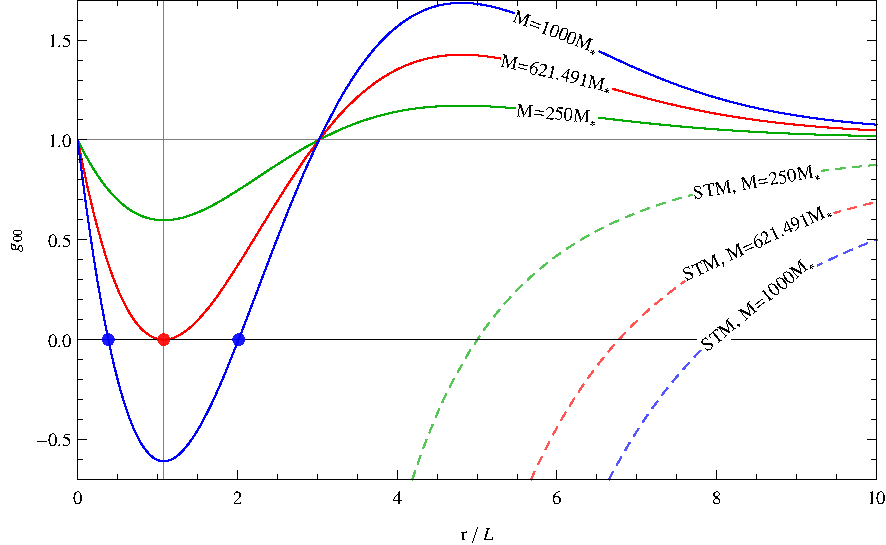
\includegraphics[scale=1]{figures/g00-n2.pdf}
\end{subfigure}
\begin{subfigure}{\textwidth}
\caption{Metric component $g_00$ for modified GUP in $n=5$ LXDs}
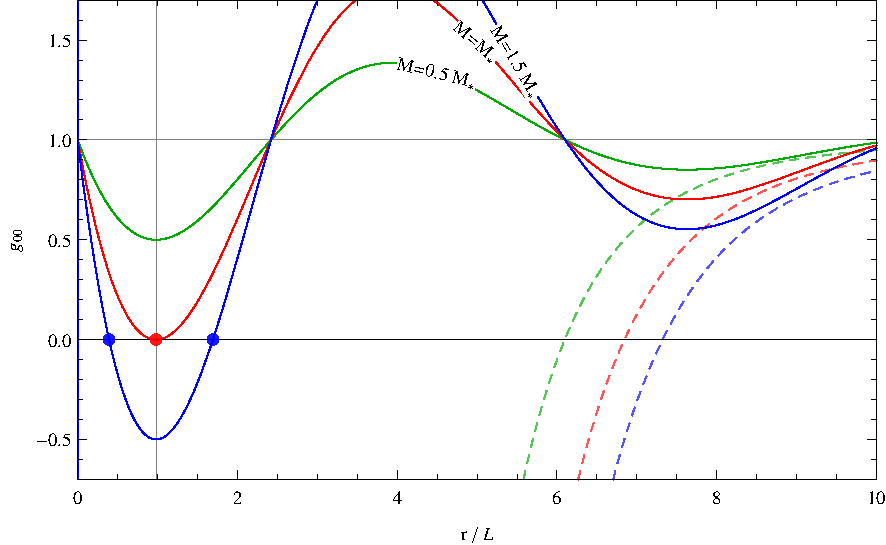
\includegraphics[scale=1]{figures/g00-n5.pdf}
\end{subfigure}
\caption{The metric behaviour for the modified GUP $[x^i, p_j] = i\delta^i_j (1+L^{2+n} p^{2+n})$ in $n$ large
extra dimensions, compared to the Schwarzschild-Tangherlini metric in $n$ large extradimensions (dashed lines).
The red dot indicates the extremal radius $r_0$, for small $r$, this metric behaves always like the $n=0$ GUP.%
}\label{fig:g00}
\end{figure}

\begin{figure}
\begin{subfigure}{\textwidth}
\centering
\caption{Temperatures of the modified GUP Black Holes}
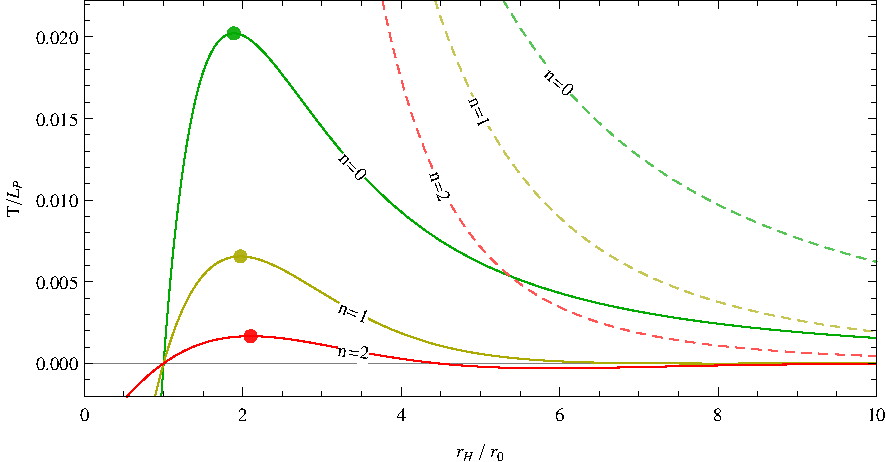
\includegraphics[scale=1]{figures/Temp.pdf}
\end{subfigure}
\begin{subfigure}{\textwidth}
\centering
\caption{Temperature of the modified GUP Black Hole in $n=7$ LXDs}
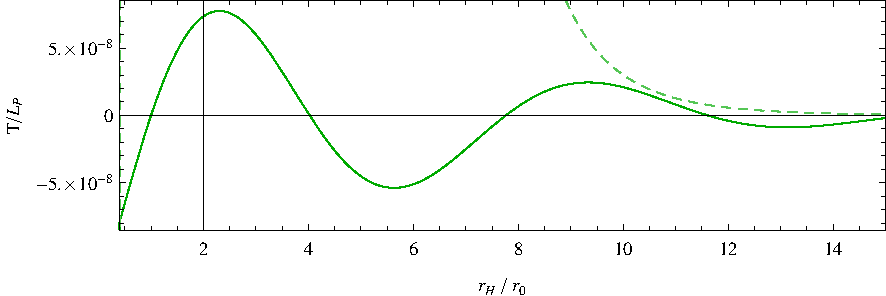
\includegraphics[scale=1]{figures/Temp-n7.pdf}
\end{subfigure}
\caption[bla]{Temperatures of the modified GUP Black holes in $n$ large extra dimensions, compared to
Schwarzschild-Black holes (dashed lines). The x-axis is scaled by the extremal radius $r_0$. In figure
(a), the circles indicate the (lowest) critical radii $r_C$ where the Heat Capacity diverges.

With increasing $n>0$, the temperature fluctuates more and more around $T=0$. The model therefore suffers
negative temperatures which have actually the same order of magnitude as the remnant temperature
for large $n$, as shown in figure (b). With each inflexion point, a diverging heat capacity is
associated. Therefore the Black holes should exhibit a rich phase structure with alternating stable
and unstable phases.
}\label{fig:temp}
\end{figure}



\newpage
\begin{thebibliography}{}
\bibitem{work}
  M.~Isi, M.~Knipfer, J.~Mureika and P.~Nicolini,
  ``Self-Completeness and the Generalized Uncertainty Principle in Extra Dimensions,'' \textit{in progress} (my latest copy: April 26, 2014).
  
\bibitem{kempf1995}
  A.~Kempf, G.~Mangano and R.~B.~Mann,
  ``Hilbert space representation of the minimal length uncertainty relation,''
  Phys.\ Rev.\ D {\bf 52} (1995) 1108
  [\href{http://arxiv.org/abs/hep-th/9412167}{hep-th/9412167}].

\bibitem{isi2013}
  M.~Isi, J.~Mureika and P.~Nicolini,
  ``Self-Completeness and the Generalized Uncertainty Principle,''
  JHEP {\bf 1311} (2013) 139
  [\href{http://arxiv.org/abs/arXiv:1310.8153}{arXiv:1310.8153 [hep-th]}].
  
  
\bibitem{NS2012}
  P.~Nicolini and E.~Spallucci,
  ``Holographic screens in ultraviolet self-complete quantum gravity,''
  Adv.\ High Energy Phys.\  {\bf 2014} (2014) 805684
  [\href{http://arxiv.org/abs/arXiv:1210.0015}{arXiv:1210.0015 [hep-th]}].
  
\bibitem{Rizzo}
  T.~G.~Rizzo,
  ``Noncommutative Inspired Black Holes in Extra Dimensions,''
  JHEP {\bf 0609} (2006) 021
  [\href{http://arxiv.org/abs/hep-ph/0606051hep-ph/0606051}{arXiv:hep-ph/0606051}].
  %%CITATION = HEP-PH/0606051;%%
  %100 citations counted in INSPIRE as of 29 Aug 2014



\end{thebibliography}

\end{document}
